\section{VM Placement Simulator}
\label{sec:injector}
%\AL[AL]{1.5 page}

The purpose of \vmps is to deliver a generic tool to evaluate new VM
placement algorithms and offer the possibility to compare
them. Concretely, it supports the management of VM creations, workload
fluctuations as well as node apparitions/removals.  Researchers can
thus focus on the implementation of new placement algorithms and
evaluate how they behave in the presence of changes that occur during
the simulation.
%
\vmps has been implemented in Java by leveraging the messaging API
(MSG) of \sg. Although the Java layer has an impact of the efficiency
of \sg, we believe its use is acceptable because Java offers important
benefits to researchers for the implementation of advanced scheduling
strategies, notably concerning the ease of implementation of new
strategies. As examples, we reimplemented the Snooze proposal in Java
and the DVMS proposal using Scala/Java.

In the following we give an overview of the framework and describe its
general functioning.% and how researchers can develop new algorithms

\subsection{Overview}
\label{sec:overview}

From a high-level view, \vmps performs a simulation in three phases:
(i) initialization (ii) injection and (iii) trace analysis (see Figure
\ref{fig:workflow}).  The initialization phase corresponds to the
creation of the environment, the VMs and the generation of the queue
of events that may represent, \eg load changes.  The
simulation is performed by at least two \sg processes, one executing
the \emph{injector}, which constitutes the generic part of the
framework, and a second one executing the to-be-simulated
\emph{scheduling algorithm}. During the simulation the scheduling
strategy is evaluated by injecting scheduling-relevant events.
\AL[MS]{This sentence above is not accurate enough I? previously it
  was : The
\emph{injector} constitutes the generic part of the framework. It
injects scheduling-relevant events during the execution of
simulations. We should reformulate}
Currently, the supported events are VM CPU load change and node
apparitions/removals that we use to simulate node crashes.



\begin{wrapfigure}{r}{.5\linewidth}
\centering
\vspace*{-.8cm}
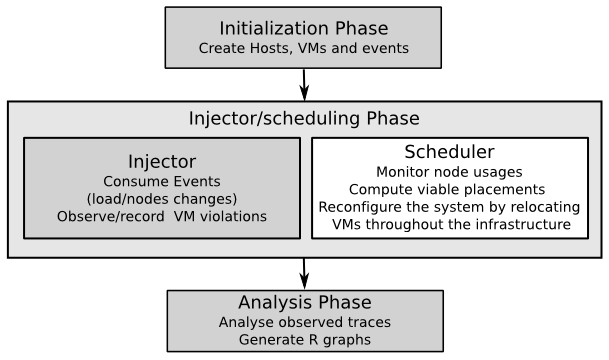
\includegraphics[width=.95\linewidth]{figures/VMPlaceS-workflow.png}
\caption{\vmps's Workflow}
{\small Gray parts correspond to the generic code while the white one
  must be provided by end-users. The current version is released with
  three different schedulers (centralized/hierarchical and distributed).}
\label{fig:workflow}
\end{wrapfigure}


% \begin{figure}
%   {\centering ~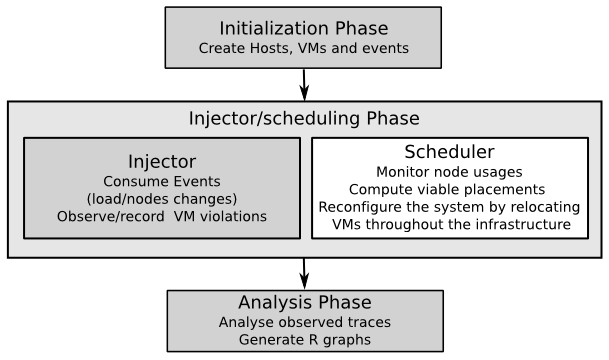
\includegraphics[width=.95\linewidth]{figures/VMPlaceS-workflow.png}}
%   \caption{\vmps's Workflow}
%   \label{fig:workflow}
% {\small Gray parts correspond to the generic code while the white one
%   must be provided by end-users. The current version is released with
%   three different schedulers (centralized/hierarchical and distributed).}
% \end{figure}

% As we describe in the next section, additional events can be easily added.
%\AL[AL]{Make two figures: a architectural one (i.e. Injector vs
 % schedulers pool and one chronological.}
%\MS{Yes, the figures are important. They could also be useful to
 % partially provide a more abstract explanation.}

Users develop their scheduling algorithm by leveraging the \sg
messaging API and a more abstract interface that is provided vy \vmps
and consists of the classes \texttt{XHost}, \texttt{XVM} and
\texttt{SimulatorManager} classes. The two former classes respectively
extend \sg's \texttt{Host} and \texttt{VM} abstractions while the
latter controls the interactions between the different components of
the VM placement simulator.  Throughout these three classes, users can
inspect, at any time, the current state of the infrastructure (\ie the
load of a host/VM, the number of VMs hosted on the whole
infrastructure or on a particular host, check whether a host is
overloaded, etc.) We have used \vmps in order to analyze three
scheduling mechanisms, cf.\ Sec.~\ref{sec:vm-schedulers}, that
represent three different software architecture models: centralized,
hierarchical and fully-distributed models for VM placement.
%% TODO
%\MS{The
%  following point is too low-level and should not come here} Although
%we do not discuss that point due to space constraints, we emphasize
%that these three mechanisms enable us to deliver concrete examples of
%how the deployment file of \sg is automatically generated by leveraging
%a generic python script.  \AL{We should highlight that point in the
%  README.org}

The last phase consists in the analysis of the collected traces in
order to gather the results of the simulation, notably by means of the
generation of figures representing, \eg resource usage statistics.

%\begin{itemize}
%\item Entropy \cite{Hermenier:2009:ECM:1508293.1508300}, a centralized approach using a constraint programming approach to solve the placement/reconfiguration VM problem;
% \item Snooze \cite{feller:ccgrid12}, a hierarchical approach where
%   each manager of a group invokes Entropy to solve the
%  placement/reconfiguration VM problem. It is noteworthy that in
%   \cite{feller:ccgrid12}, Snooze is using a specific heuristic to solve the placement/reconfiguration VM problem. As the sake of simplicity, we have simply reused the entropy scheduling code.
%\item  DVMS \cite{quesnel:cpe2012}, a distributed approach that dynamically partitions the system and invokes Entropy on each partition.
% \end{itemize}

\subsection{Initialization Phase}

In the beginning, \vmps creates $n$ VMs and assigns them in a
round-robin manner to the first $p$ hosts defined in the platform
file.  The default platform file corresponds to a cluster of $h+s$
hosts, where $h$ corresponds to the number of hosting nodes and $s$ to
the number of services nodes. The values $n$, $h$ and $s$ constitute
input parameters of the simulations (specified in a Java property
file).
%% TODO
% \AL[AL]{Update the size of the cluster autonomically by
%  leveraging p + s}
These hosts are organized in form of topologies, a cluster topology
being the most common ones. It is possible, however, to define more
complex platforms to simulate, for instance, scenarios involving
federated data centers.
%Note that $s$ can be equals to 0 if the
%scheduling strategy is directly executed on the hosting nodes.

Each VM is created based on one of the predefined VM classes. A VM
class corresponds to a template specifying the VM attributes and its
memory footprint. Concretely, it is
% described as
% \texttt{nb\_cpu:ramsize:net\_bw:mig\_speed:mem\_speed}
defined in terms of five parameters: the number of cores
\texttt{nb\_cpus}, the size of the memory \texttt{ramsize}, the
network bandwidth \texttt{net\_bw}, the maximum bandwidth available
migrate it \texttt{mig\_speed} and the maximum memory update speed
\texttt{mem\_speed} when the VM is consuming 100\% of its CPU
resources. As pointed out in Section \ref{sec:sg}, the memory update
speed is a critical parameter that governs the migration time as well
as the amount of transferred data. By giving the possibility to define
VM classes, \vmps allows researchers to simulate different kinds of
workload (\ie memory-intensive vs non-intensive workloads), and thus
analyze more realistic Cloud Computing problems.  Available classes
are defined in a specific text file that can be modified according to
the user's needs.
%\MS{Follows a low-level mechanism!}
% TODO not addressed yet. This text should appear in the README
%At creation time
%of a VM, a process selects one class (\ie one line) in the file
%randomly. Hence, if a user wants to favor a specific class, he can
%simply repeat the line of the class several times.
%
Finally, all VMs start with a CPU consumption of 0 that will evolve
during the simulation in terms of the injected load as explained
below.

Once the creation and the assignment of VMs completed, \vmps spawns at
least two SG processes, the \emph{injector} and the launcher of the
selected scheduler.  The first action of the \emph{injector} consists
in creating the different event queues and merge them into a global
one that will be consumed during the second phase of the simulation.
For now, we generate two kinds of event: \emph{CPU load} and
\emph{node crash} events.
%\todo{Before apparitions/ removals}
% The former consists in changing the load of a VM by creating and
% assigning a new \sg task in the VM while the second aims at
% simulating crashes.
%
% Changing the load of a VM has a direct impact of its memory update
% speed and thus on the time to migrate it between two hosts.
The \emph{CPU load} event queue is generated in order to change the
load of each VM every $t$ seconds on average. $t$ is a random variable
that follows an exponential distribution with rate parameter
$\lambda_t$ while the CPU load of a VM evolves according to a Gaussian
distribution defined by a particular mean ($\mu$) as well as a
particular standard deviation ($\sigma$). $t$, $\mu$ and $\sigma$ are
provided as input parameters of a simulation.  As the CPU load can
fluctuate between 0 and 100\%, \vmps prevents the assignment of
nonsensical values when the Gaussian distribution returns a number
smaller than 0 or greater than 100. Although this has no impact on the
execution of the simulation, we emphasize that this can
reduce/increase the effective mean of the VM load, especially when
$\sigma$ is high.  Hence, it is important for users to specify
appropriate values.
%% TODO
%\AL[AL]{A binomial law would have solved this issue: too late too bad :(}
%Although this can have an impact on the
%effective mean, especially when $\sigma$ is high, we believe it was
%non appropriated to request it is easier for end-users to specify $\mu$ and
%$\sigma$ parameters than
Furthermore, each random process used in \vmps is initialized with a
seed that is defined in a configuration file. This way, we can ensure
that different simulations are reproducible and may be used to
establish fair comparisons.

The \emph{node crash} event queue is generated in order to turn off a
node every $f$ seconds on average for a duration of $d$ seconds.
Similarly to the $t$ value above, $f$ follows an exponential
distribution with rate $\lambda_f$. $f$ and $d$ are also provided as
input parameters of a simulation.

Adding new events can easily be done by simply defining new event Java
classes implementing the \texttt{InjectorEvent} interface and by
adding the code in charge of generating the associated queue. Such a
new queue will be merged into the global one and its events will then be
consumed similarly to other ones during the \emph{injector phase}.

\subsection{Injector Phase}

Once the VMs and the global event queue are ready, the evaluation of
the scheduling mechanism can start. First, the injector process
iteratively consumes the different events that represent, for now,
load changes of a VM or turning a node off or on. Changing the load of
a VM corresponds to the creation and the assignment of a new \sg task
in the VM. This new task has a direct impact on the time that will be
needed to migrate the VM as it increases or decreases the current CPU
load and thus% the percentage of
its memory update speed.
% \MS[AL]{Is the above paragraph clear enough?}
% that is indicated by the \texttt{mem\_speed}
%% parameter given in the class description.
When a node is turning off, the VMs that were running on that node are
temporarily discarded, \ie they are hidden and cannot be accessed
until the node comes back to life. This way, the scheduler cannot
handle them.
 %\AL[AL, MS, JP]{This is ugly but unfortunately the true,
 % it will be better to reassign those VMs on other nodes, but which
 % one?  }
We leave for future work other approaches that can better
match realistic scenarios such as turning off the VMs and
reprovisioning them on other nodes.
%

As defined by the scheduling algorithm, VMs will be suspended/resumed
or relocated on the available hosts to meet scheduling objectives and
SLA guarantees.  Note that users must implement the algorithm in
charge of solving the VMPP but also the code in charge of applying
reconfiguration plans by invoking the appropriate methods available
from the \texttt{SimulatorManager} class. This step is essential as
the reconfiguration cost is a key element of dynamic placement
systems.

% \MS[AL]{maybe it is better to prevent the access to Xhost
%   and XVM methods that can change the Simulator States. Hence, we
%   should enforce the access only through the SimulatorManager class?
%   What do you think? Yes, would be cleaner. Can we just present the
%   interface as such? Or not talk about the direct possibility?}
Last but not least, it is noteworthy that \vmps really invokes the
execution of each scheduling strategy in order to get the effective
reconfiguration plan.  That is, the computation time that is observed
is not simulated but corresponds to the effective one, only the
workload inside the VMs and the migration operations are simulated in
\sg. It is hence mandatory to propagate the reconfiguration time into
the \sg engine.%
% The following is IMO a technical detail
% by invoking a \texttt{wait} call of the MSG interface.

\subsection{Trace Analysis}
\label{subsec:traces-analysis}

The last step of \vmps consists in analyzing the information that has
been collected during the simulation.
% in order to understand and compare the behavior of the different
% algorithms.
This analysis is done in two steps. First, \vmps records several
metrics related to the platform utilization throughout the simulation
by leveraging an extended version of \sg's TRACE
module\footnote{\url{http://simgrid.gforge.inria.fr/simgrid/3.12/doc/tracing.html}}.
This way, visualization tools that have been developed by the \sg
community, such as PajeNG~\cite{pageng:www}, may be used. Furthermore,
our extension enables the creation of a trace file in the JSON file
format, which is used to generate several figures using the R
statistical environment~\cite{R:Bloomfield:2014} about the resource
usage during the simulation.

By default, \vmps records the load of the different VMs and hosts, the
appearance and the duration of each violation of VM requirements in
the system, the number of migrations, the number of times the
scheduler mechanism has been invoked and the number of times it
succeeds or fails to resolve non-viable configurations.
%
Although these pieces of information are key elements to understand
and compare the behavior of the different algorithms, we emphasize
that the TRACE API enables the creation of as many variables as
necessary, thus allowing researchers to instrument their own algorithm
with specific variables that record other pieces of information.
